\documentclass[SoftwareDesign/SoftwareDesign_main.tex]{subfiles}

\begin{document}
\section{Design af CarnGo Database}
I dette afsnit beskrives designet af databasen. Databasens operationer og funktionalitet tager udgangspunkt i beskrivelsen i afsnit X i softwarearkitekturen. Databasen er designet ud som relationel model, hvor relationer kan sammenlignes med hinanden. Figur \ref{fig:ERDiagram} er et E/R diagram, som er til værktøj til at modellere databasen - det viser alle entiteter og deres relationerne. En af de vigtigste elementer for databasen, er at tilgå samme data ved samtidigt at opretholde dataens integritet, som beskrives senere i dette afsnit. E/R diagrammet repræsenteres ved Chens notation. 
\begin{figure}[H]
    \centering
    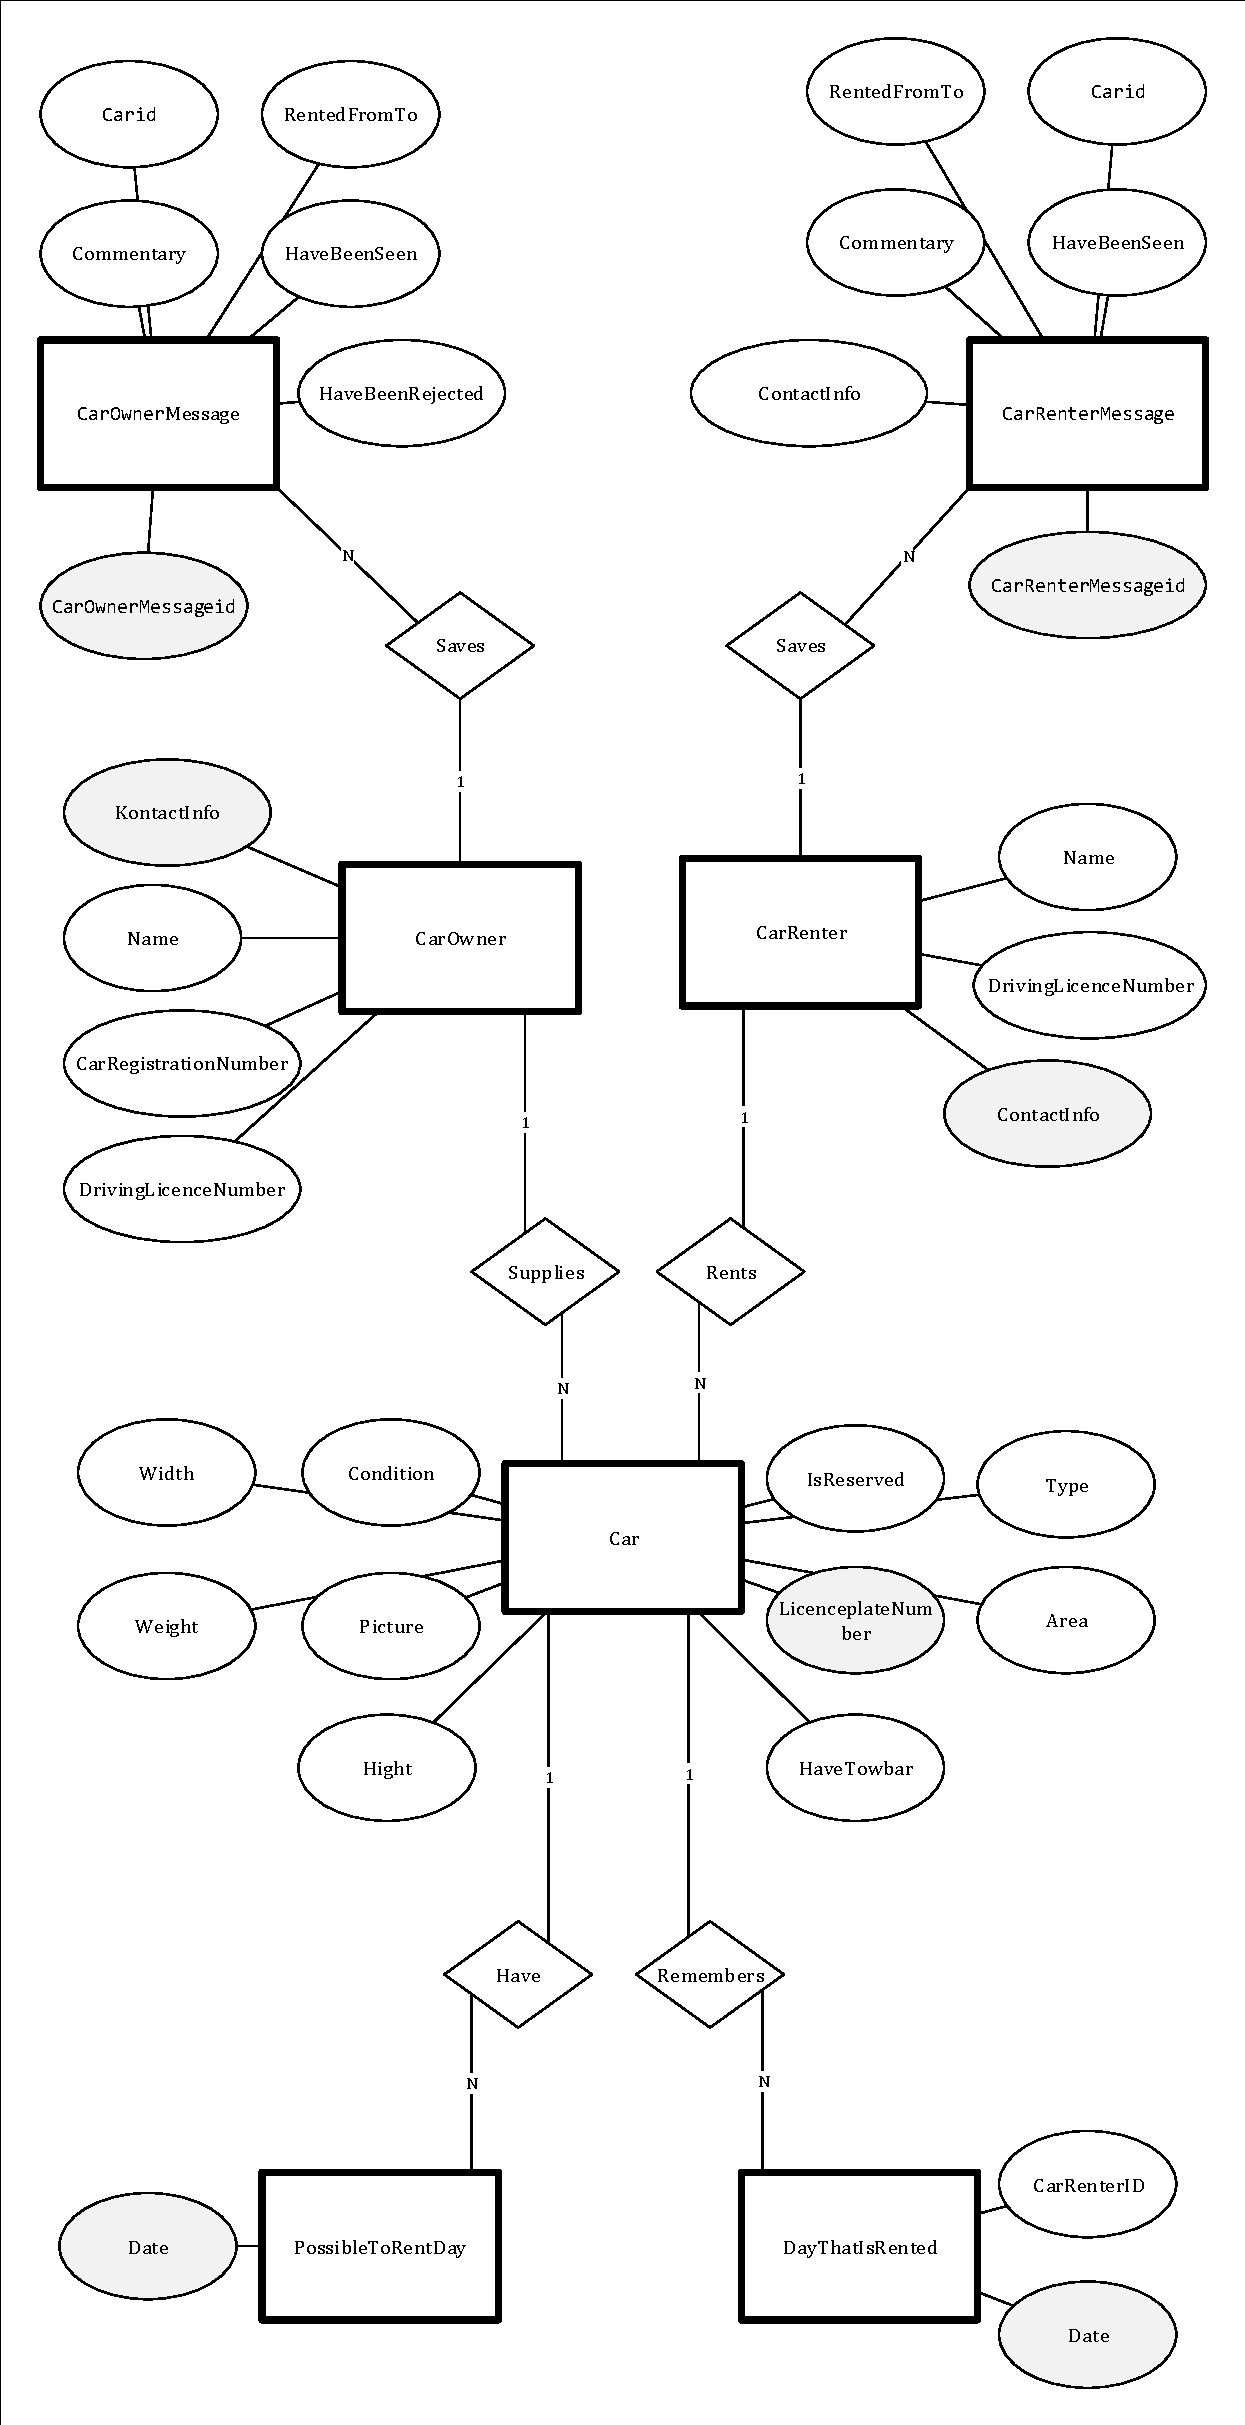
\includegraphics[width=0.9\textwidth]{Arkitektur/Softwarearkitektur/Database/graphics/ER.pdf}
    \caption{Entity–relationship diagram for CarnGO databasen}
    \label{fig:ERDiagram}
\end{figure}
Databasen ligger på en ekstern server og tilgås via SQL server query's, automatisk genereret af "entity framework" ud fra funktioner i en klasse af typen DbContext. Disse funktioner kaldes via funktioner i model laget. En vigtig overvejelse er hvordan man kan tage mindst muligt af databasens kapacitet. Siden det tager mere tid at finde mange små elementer og hente dem ned, end at tage et større element, er det ønskeligt at lave større query's, frem for mange query's.

Dette betyder at hvis data kan arbejdes med lokalt fortrækkes dette indtil alle ændringer af data er færdige, og derefter opdatere vi databasen.
For data der kun ændres af brugeren som ser det, for eksempel CarOwner som laver ændringer i CarOwnerMessage men ikke sender den endnu kan GUI'en opdateres med det nye data i viewmodellen, allerede inden dataet sendes til databasen og det er derfor først nødvendigt at opdatere databasen, når en kladde skal gemmes eller beskeden er færdig.

En udfordring opstår dog når data kan ændres af en anden bruger. En ny bil kunne være sat til leje mens en lejer kigger på listen over biler der kan lejes, eller en lejer kunne have sent en besked til en udlejer mens denne var på deres profil. Her er GUI'en ikke synkroniseret og brugeren får vist forældet data.
Udfordringen er hvornår og hvor tit dataet skal opdateres.

Man kunne tjekke databasen oftere end brugeren kan læse data fra skærmen, og derved have en effektivt helt synkroniseret GUI. Dette vil dog kræve enormt mange query's per sekund, og blot få brugere som er logget på CarnGo samtidig vil overbelaste databasen. Man må derfor vælge en længere tid mellem opdateringerne, men hvis man vælger en større tid, for eksempel 5 minutter, så kan brugeren bevæge sig rundt på de forskellige dele af GUI'en og få forkerte data. Dette er særligt slemt for data brugeren selv har ændret. En bruger som lige har delvist skrevet og gemt en besked, og derefter vil skrive videre på den og bliver informeret om at denne ikke findes vil begynde at agere ud fra denne forkerte information. Det er vanskeligt at vælge et passende interval.

Man kan også tjekke databasen når bestemte begivenheder sker. Når brugeren skifter til en ny del af GUI'en som kræver brug af data fra databasen, eller når brugeren ændre data. Derved vil meget aktive brugere få opdateret data ofte, og mindre aktive brugere vil få opdatere data mindre ofte, og dette er selvregulerende med brugerens aktivitet. 

Der er valgt en kombineret løsning, hvor vi opdatere databasen ved bestemte begivenheder, og hver gang det gøres, nulstillet en timer. Hvis timeren når 10 minutter opdateres serveren og GUI.


\end{document}